\documentclass[12pt]{article}

% ── Packages ──────────────────────────────────────────────────────────────────
\usepackage[margin=1in]{geometry}
\usepackage{amsmath, amssymb}
\usepackage{graphicx}
\usepackage{booktabs}
\usepackage{array}
\usepackage{hyperref}
\usepackage{caption}
\usepackage{subcaption}
\usepackage{float}
\usepackage{xcolor}
\usepackage{svg}

% ── Metadata ──────────────────────────────────────────────────────────────────
\title{CSA SAR Imaging: Simulation Method}
\author{Jen-Tse Chen}
\date{\today}

% ── Helpers ───────────────────────────────────────────────────────────────────
\newcommand{\rect}{\operatorname{rect}}

% ──────────────────────────────────────────────────────────────────────────────
\begin{document}
\maketitle
\tableofcontents
\newpage

% ══════════════════════════════════════════════════════════════════════════════
\section{Simulation Setup}
% ══════════════════════════════════════════════════════════════════════════════

\subsection{Signal Model}

\subsubsection{Chirp Echo Signal}

The multi-target scattering model of the chirp echo signal is represented as a
matrix $S = [s_{m,n}]_{M \times N}$, where:

\begin{itemize}
    \item $\eta = m\Delta\eta$: slow time
    \item $\tau = n\Delta\tau$: fast time
    \item $A_k$: scattering coefficient of point target $k$
    \item $R_k(m\Delta\eta) = \sqrt{(R_0 + \Delta R_{0,k})^2 +
          (m\Delta\eta + \Delta\eta_k)^2 V_r^2}$, where
          \begin{itemize}
              \item $\Delta R_{0,k}$: slant-range offset from target $k$ to scene centre
              \item $\Delta\eta_k$: azimuth time offset from target $k$ to scene centre
          \end{itemize}
\end{itemize}

\begin{equation}
    s_{m,n} = \sum_k A_k
    \rect\!\left(\frac{n\Delta\tau - \frac{2R_k(m\Delta\eta)}{c}}{T_r}\right)
    \cdot e^{\,j\pi\frac{B_r}{T_r}\left(n\Delta\tau - \frac{2R_k(m\Delta\eta)}{c}\right)^2}
    \cdot e^{-j4\pi\frac{R_k(m\Delta\eta)}{\lambda}}
\end{equation}

\subsubsection{Coherent Scattering}

\paragraph{Time-Domain Model}

Coherent scattering applied in the time domain:
\begin{equation}
    S \circ C + W, \quad C = [c_{m,n}]_{M\times N},\quad c_{m,n} = e^{j\theta_{m,n}},
    \quad \theta_{m,n} \sim \mathcal{U}(0, 2\pi)
\end{equation}

\paragraph{Spatial-Domain Model}

Coherent scattering applied in the spatial (image) domain:
\begin{equation}
    T(S + W) \circ C, \quad c_{m,n} \sim \mathcal{E}(1)
\end{equation}
where $T(\cdot)$ denotes the imaging algorithm (e.g.\ RDA or CSA).

\subsubsection{Thermal Noise}

Thermal noise is modelled as a complex Gaussian matrix
$W = [w_{m,n}]_{M\times N}$ with $w_{m,n} \sim \mathcal{CN}(0,\sigma)$:

\begin{align}
    \sigma^2 &= P_n / 2 \\
    P_n &= P_s / \mathrm{SNR} \quad \text{(instantaneous noise power)} \\
    P_s &= \Re\{x[n]\}^2 + \Im\{x[n]\}^2 \quad \text{(instantaneous signal power)}
\end{align}

\subsection{Image-to-Echo Conversion}

Given a pixel displacement $d_i$ in the ground-range direction and the
geometry $R_0^2 = H^2 + G^2$, the slant-range to the displaced pixel is
$R_0' = \sqrt{H^2 + (G + d_i)^2}$. A Taylor expansion gives:

\begin{align}
    R_0' - R_0
    &= \sqrt{H^2 + (G+d_i)^2} - R_0 \notag \\
    &= \sqrt{R_0^2 + 2Gd_i + d_i^2} - R_0 \notag \\
    &\approx R_0\!\left(1 + \frac{2Gd_i + d_i^2}{2R_0^2}\right) - R_0
       \quad \text{(first-order Taylor)} \notag \\
    &= \frac{2Gd_i + d_i^2}{2R_0} \notag \\
    &\approx \frac{G d_i}{R_0}
       \quad \text{($d_i \ll G$)} \notag \\
    &\approx d_i
       \quad \text{($G \approx R_0$)}
\end{align}

Therefore $R_0' \approx R_0 + d_i$.


\subsection{Simulation Parameters}

\begin{table}[H]
    \centering
    \caption{Simulation parameter definitions.}
    \begin{tabular}{>{\ttfamily}lp{0.6\textwidth}}
        \toprule
        \normalfont Parameter & Description \\
        \midrule
        wavelength\_m           & Carrier wavelength (m) \\
        pulse\_width\_sec        & Pulse duration (s) \\
        pulse\_rep\_freq\_hz     & Pulse repetition frequency (Hz) \\
        bandwidth\_hz           & Range chirp bandwidth (Hz) \\
        sampling\_freq\_hz      & Range sampling frequency (Hz) \\
        closest\_slant\_range\_m & Closest slant range to scene centre (m) \\
        azi\_win\_en            & Enable azimuth window (beam pattern) \\
        rng\_pad\_time          & Range padding factor; row length $= T_r \cdot f_s \cdot \mathtt{rng\_pad\_time}$ \\
        noise\_en               & Enable additive thermal noise \\
        snr\_db                 & SNR in dB (ignored when \texttt{noise\_en} is \texttt{False}) \\
        \bottomrule
    \end{tabular}
\end{table}

% ══════════════════════════════════════════════════════════════════════════════
\section{Umbra Image Denoising}
% ══════════════════════════════════════════════════════════════════════════════

\subsection{Processing Flow}

All methods start by normalising the float SAR slice to uint8 $[0, 255]$ via
min-max scaling, which is required by the OpenCV processing functions.
The pipeline then diverges by method:

\begin{itemize}
    \item \textbf{Raw} — no processing; the normalised slice is used as-is.
    \item \textbf{Binary} — a fixed threshold is applied; pixels above the
          threshold are set to 1, others to 0.
    \item \textbf{Otsu} — same as binary, but the threshold is computed
          automatically by minimising intra-class intensity variance.
    \item \textbf{Filter methods} (Bilateral, Guided, TV, Lee) — a denoising
          filter is applied first to suppress speckle, then Otsu thresholding
          is run on the smoothed image to produce a cleaner binary mask.
\end{itemize}

For filter methods, the role of the filter is to improve the quality of the
subsequent Otsu threshold: speckle in raw SAR creates a noisy intensity
histogram, causing Otsu to produce a ragged mask. Denoising first yields two
cleaner histogram peaks (target vs.\ clutter) so the threshold is more reliable.

After thresholding, morphological closing is optionally applied to fill small
holes inside detected regions.

\subsection{Morphological Closing}

Morphological closing is a two-step operation applied to a binary image:

\begin{enumerate}
    \item \textbf{Dilation} — expands bright regions by adding pixels around their edges.
    \item \textbf{Erosion} — shrinks the dilated regions back by removing pixels around their edges.
\end{enumerate}

The net effect is that small gaps and holes within detected regions are filled and nearby
disconnected blobs are merged, while the overall shape and size remain roughly unchanged.
Formally, closing of image $I$ by structuring element $B$ is defined as:

\begin{equation}
    I \bullet B = (I \oplus B) \ominus B
\end{equation}

where $\oplus$ denotes dilation and $\ominus$ denotes erosion.

In the SAR context, after thresholding or denoising produces a rough binary mask,
morphological closing fills small dark holes inside a detected target
(e.g.\ a ship) that were incorrectly zeroed out, yielding a more solid and
contiguous detection region.

\subsection{Results}

\begin{figure}[H]
    \centering
    \begin{subfigure}[b]{0.48\textwidth}
        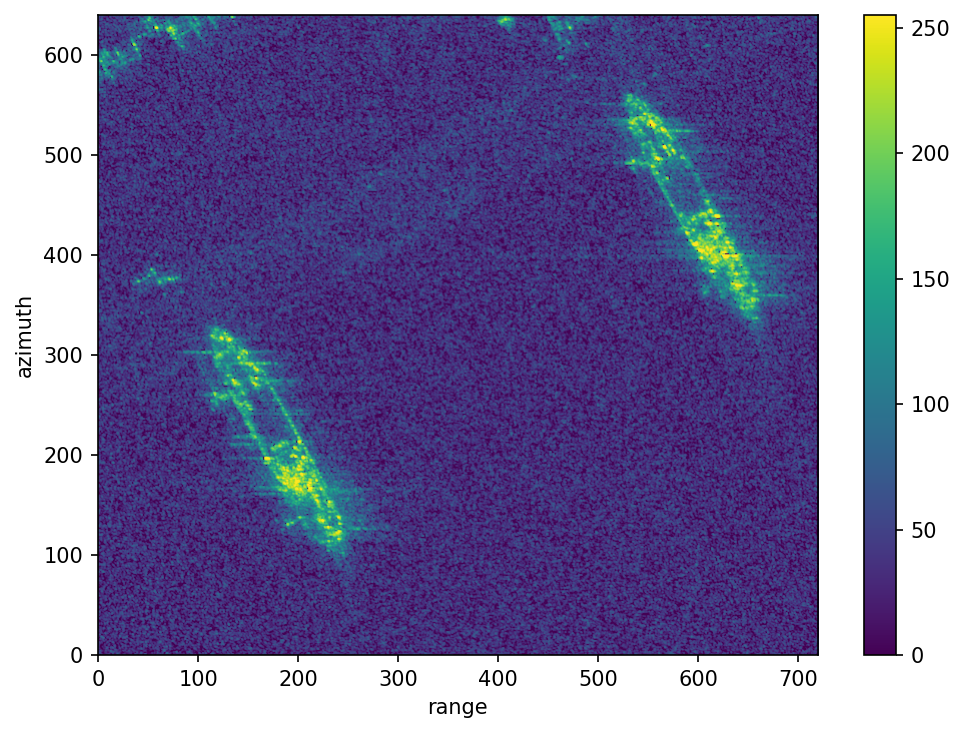
\includegraphics[width=\textwidth]{../../diagram/umbra_image_denoising/tsoying_naval_base_raw.png}
        \caption{Raw image.}
    \end{subfigure}
\end{figure}

\begin{figure}[H]
    \centering
    \begin{subfigure}[b]{0.48\textwidth}
        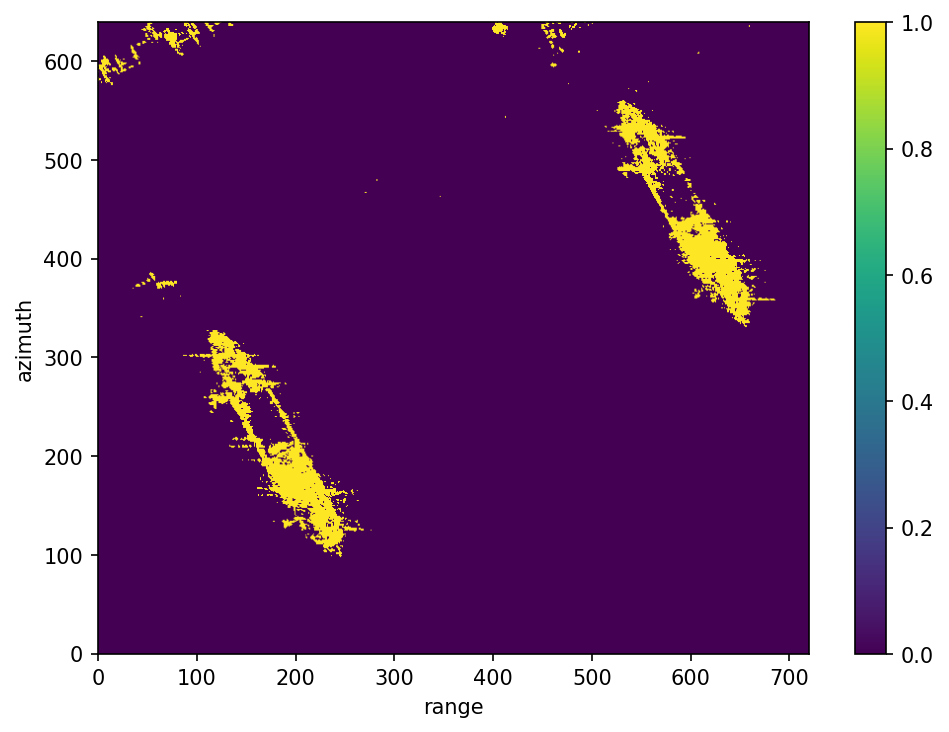
\includegraphics[width=\textwidth]{../../diagram/umbra_image_denoising/tsoying_naval_base_binary.png}
        \caption{Binary thresholding.}
    \end{subfigure}
    \hfill
    \begin{subfigure}[b]{0.48\textwidth}
        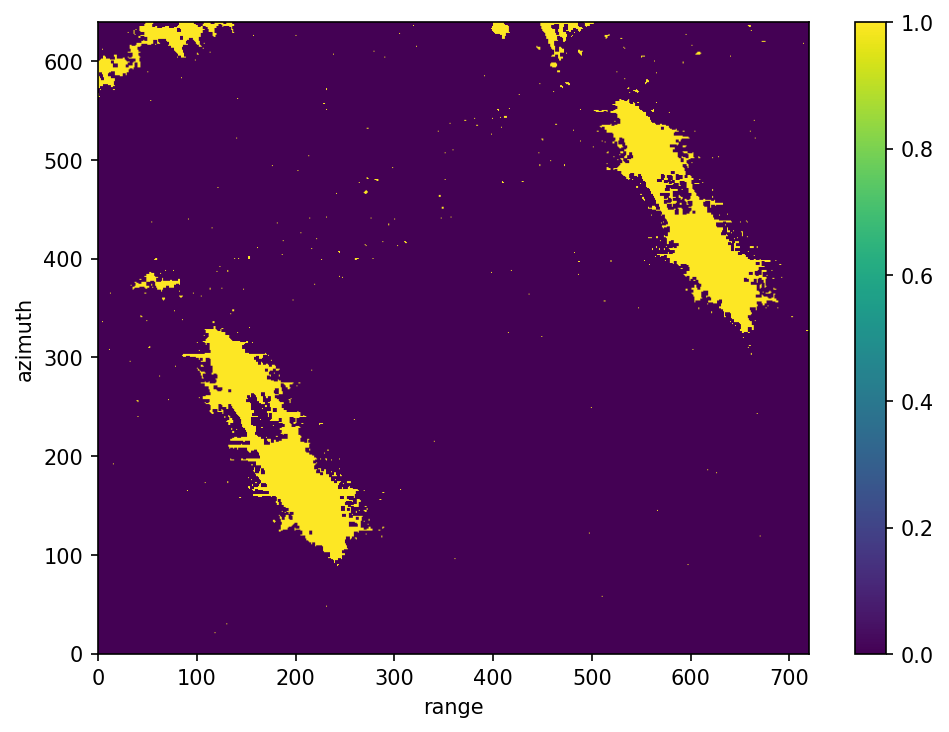
\includegraphics[width=\textwidth]{../../diagram/umbra_image_denoising/tsoying_naval_base_otsu.png}
        \caption{Otsu thresholding.}
    \end{subfigure}
\end{figure}

\begin{figure}[H]
    \centering
    \begin{subfigure}[b]{0.48\textwidth}
        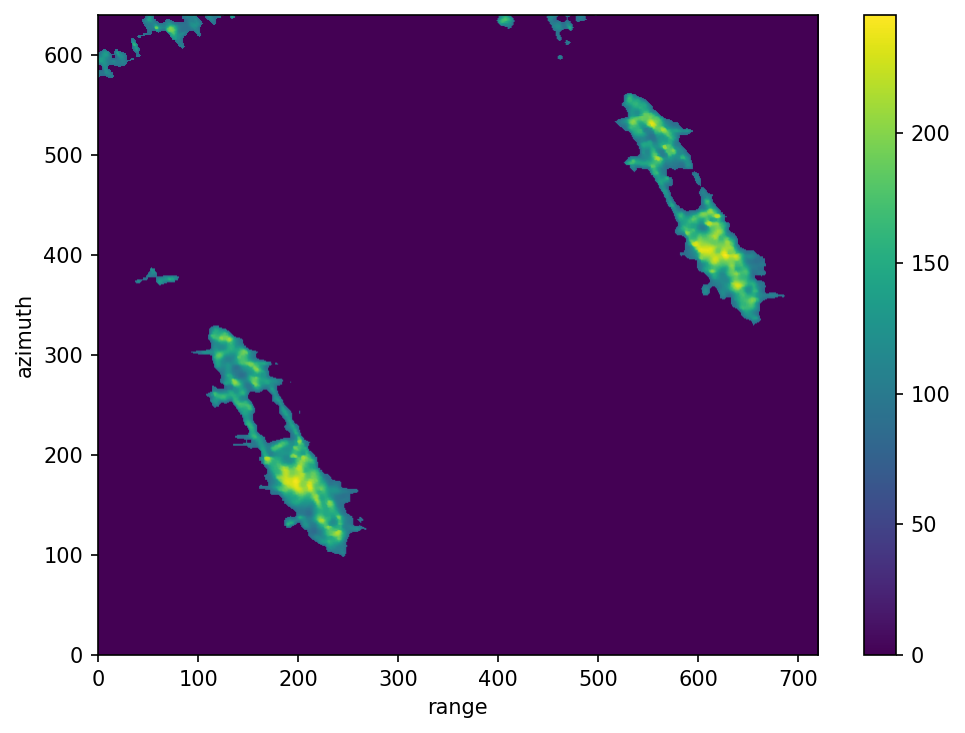
\includegraphics[width=\textwidth]{../../diagram/umbra_image_denoising/tsoying_naval_base_bilateral.png}
        \caption{Bilateral filter.}
    \end{subfigure}
    \hfill
    \begin{subfigure}[b]{0.48\textwidth}
        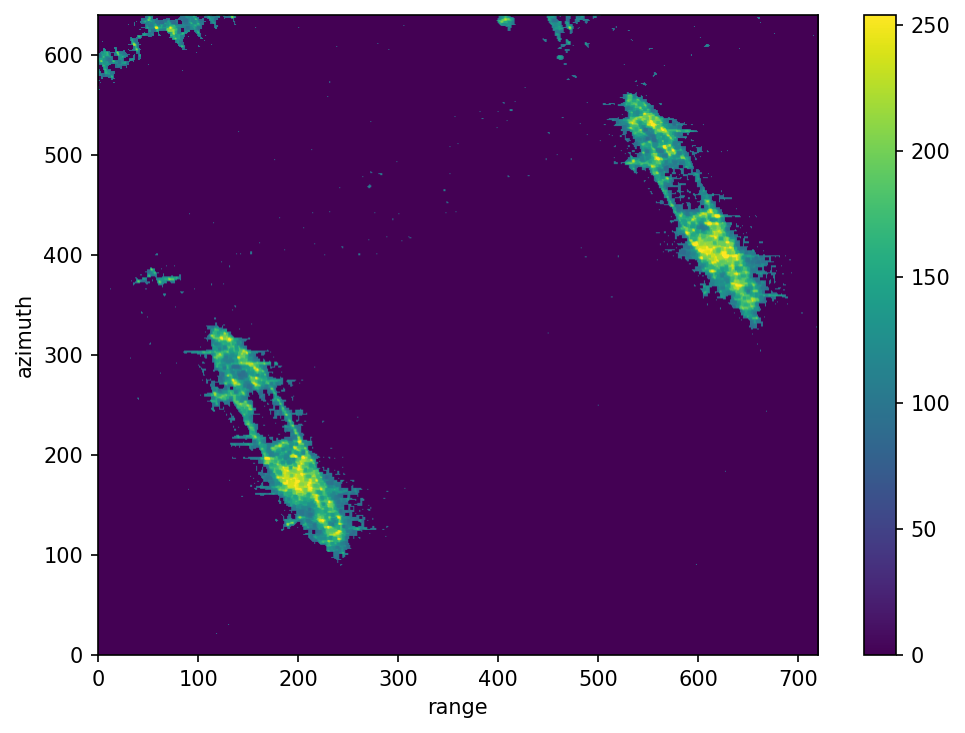
\includegraphics[width=\textwidth]{../../diagram/umbra_image_denoising/tsoying_naval_base_guided.png}
        \caption{Guided filter.}
    \end{subfigure}
\end{figure}

\begin{figure}[H]
    \centering
    \begin{subfigure}[b]{0.48\textwidth}
        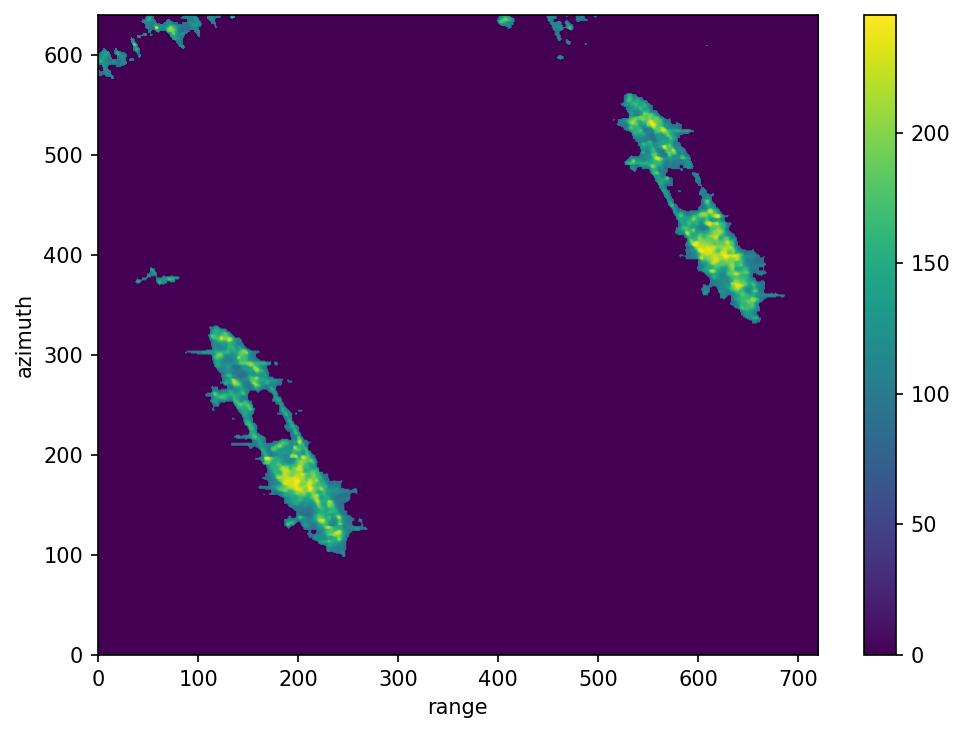
\includegraphics[width=\textwidth]{../../diagram/umbra_image_denoising/tsoying_naval_base_tv.png}
        \caption{Total variation filter.}
    \end{subfigure}
    \hfill
    \begin{subfigure}[b]{0.48\textwidth}
        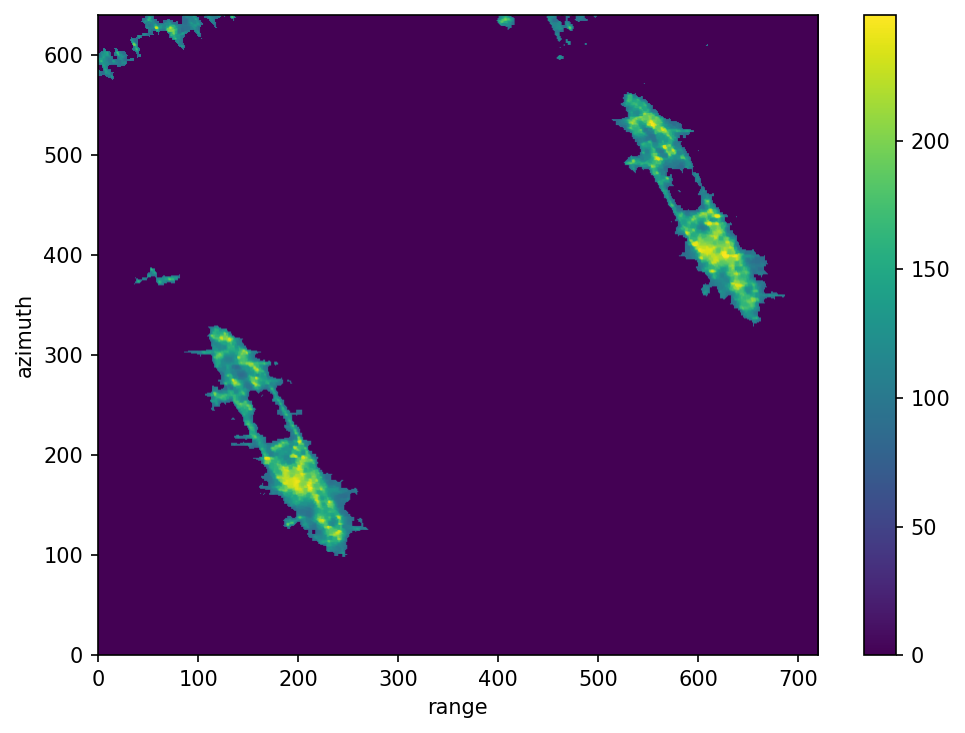
\includegraphics[width=\textwidth]{../../diagram/umbra_image_denoising/tsoying_naval_base_lee.png}
        \caption{Lee filter.}
    \end{subfigure}
\end{figure}

\begin{table}[H]
    \centering
    \caption{Non-zero sample counts per denoising method.}
    \begin{tabular}{lr}
        \toprule
        Method & Non-zero samples \\
        \midrule
        Raw SAR Image & 443,448 \\
        Binary Thresholding (threshold = 110) & 16,419 \\
        Otsu's Thresholding + Morphological Closing & 27,572 \\
        Bilateral Filter + Morphological Closing & 23,629 \\
        Guided Filter + Morphological Closing & 27,087 \\
        Total Variation (TV) Filter + Morphological Closing & 23,075 \\
        Lee Filter + Morphological Closing & 23,873 \\
        \bottomrule
    \end{tabular}
\end{table}


% ══════════════════════════════════════════════════════════════════════════════
\section{Performance Metrics}
% ══════════════════════════════════════════════════════════════════════════════

All metrics are computed after converting both images to dB scale and applying
peak-to-peak$-30$\,dB normalisation to $[0,1]$.

\subsection{Structural Similarity Index (SSIM)}

\begin{equation}
    \text{SSIM} = L \cdot C \cdot S
\end{equation}

\paragraph{Luminance}
\begin{equation}
    L(x,y) = \frac{2\mu_x\mu_y + C_1}{\mu_x^2 + \mu_y^2 + C_1}
\end{equation}
Compares local mean brightness; $C_1 = (0.01 \cdot d)^2$.

\paragraph{Contrast}
\begin{equation}
    C(x,y) = \frac{2\sigma_x\sigma_y + C_2}{\sigma_x^2 + \sigma_y^2 + C_2}
\end{equation}
Compares local standard deviation; $C_2 = (0.03 \cdot d)^2$.

\paragraph{Structure}
\begin{equation}
    S(x,y) = \frac{\sigma_{xy} + C_3}{\sigma_x\sigma_y + C_3}
\end{equation}
Normalised cross-covariance (Pearson correlation of patch values); $C_3 = C_2/2$.

\subsection{PSNR and MSE}

\begin{equation}
    \text{PSNR} = 20\log_{10}\!\left(\frac{1}{\sqrt{\text{MSE}}}\right) \text{ dB},
    \qquad
    \text{MSE} = \frac{1}{N}\sum_i (x_i - y_i)^2
\end{equation}

\subsection{Signal-to-Clutter Ratio (SCR)}

\begin{equation}
    \text{SCR} = 10\log_{10}\!\left(\frac{\bar{P}_{\text{signal}}}{\bar{P}_{\text{clutter}}}\right) \text{ dB}
\end{equation}

The brightest pixel is taken as the target centre. An inner disk of radius
$r_1 = 5$\,px defines the \emph{signal zone}; an annulus between $r_1$ and
$r_2 = 15$\,px defines the \emph{clutter zone}.

\subsection{Image Entropy}

\begin{equation}
    E = -\sum_{i=1}^{M}\sum_{j=1}^{N} P_{i,j}\ln P_{i,j},
    \qquad P_{i,j} = \frac{|I_{i,j}|^2}{\displaystyle\sum_{i,j}|I_{i,j}|^2}
\end{equation}

\noindent where $\lim_{P\to 0} P\ln P = 0$ by convention.

% ══════════════════════════════════════════════════════════════════════════════
\section{Results}
% ══════════════════════════════════════════════════════════════════════════════

\subsection{Metric Summary}

\begin{table}[H]
    \centering
    \caption{Performance metrics (last updated 2026-04-11).}
    \begin{tabular}{lccc}
        \toprule
        Metric & threshold $= 0$ & threshold $= 2\times10^5$ \\
        \midrule
        SSIM            & 0.33491 & 0.03021 \\
        Luminance $L$   & 0.89509 & 0.06166 \\
        Contrast $C$    & 0.69948 & 0.15396 \\
        Structure $S$   & 0.49793 & 0.94501 \\
        PSNR (dB)       & 10.81   & 3.40    \\
        MSE $[0,1]$     & 0.08305 & 0.45706 \\
        SCR result (dB) & 0.78    & 1.04    \\
        \bottomrule
    \end{tabular}
\end{table}

\subsection{SSIM Component Interpretation}

\begin{table}[H]
    \centering
    \caption{SAR interpretation of each SSIM component.}
    \begin{tabular}{lll}
        \toprule
        Component & SAR Interpretation & Role in Object Detection \\
        \midrule
        Luminance $L$ & Average backscatter &
            Distinguishes overall brightness; secondary to shape. \\
        Contrast $C$ & Variance / intensity &
            Separates target signal from background clutter. \\
        Structure $S$ & Spatial correlation &
            Primary metric; defines shape, prevents false alarms. \\
        \bottomrule
    \end{tabular}
\end{table}

\end{document}
